% !TEX root = ../utltcp-paper.tex


%The results of scientific research should be reproducible.
Scientific research manuscripts should contain sufficient algorithmic and methodological details so that
%independent implementations can be made that replicates the results
experiments may be independently replicated, and results validated \cite{munafo:2017:manifesto}. 
For computer networking papers, such as this, reproducibility is facilitated by the source code used in generation of
the results, along with details of the environment used for
testing. This appendix describes the technical details
%approach to ensuring reproducibility of our results,
to reproduce our evaluations, including artefacts and assumptions.

% FIXME: should likely expand the discussion of the implementation, but
% there probably isn't space

We implemented TCP Hollywood in the Linux kernel, version 3.18. The TCP
modifications in the kernel impact approximately 300 lines of code, while
the intermediary layer is comprised of around 600 lines of user-space C
code. The design is described in Section \ref{sec:design}, and the source
code is available at ~\cite{hollywood-src}.
Our experiments used version \texttt{0bb4a643cdde26241f3807c4d5b3987d97be7f66}
of the \texttt{git} repository, dated 17 January 2017.

Our evaluations were designed to validate the analysis presented in Section \ref{sec:analysis}, and
determine whether TCP Hollywood performs as expected in the scenarios described. Simultaneously, a real-world implementation was needed to facilitate deployment,
%although we do conduct real-world evaluations of deployment
as assessed in Section \ref{sec:deployability}.
%There were a number of viable options for conducting the performance
The list of viable options for evaluations in Section \ref{sec:perfeval}
%. These
included real-world measurements on the public Internet, measurements using
network emulation testbed hardware, and software simulations. The need to
validate our analysis meant that any testing environment be tightly controlled.
This ruled out the use of real-world measurements for our performance
evaluations, due to the unpredictable nature of the cross traffic in the public
Internet. Additional control can be achieved via network emulation testbeds.
However, this comes at the cost of flexibility, since hardware and software
reconfiguration is needed to test different network conditions. Our desire for
control and flexibility could only be achieved with software.
% emulation or simulation, gives flexibility to change the scenarios
% being studied, while still giving control of the environment,

For our purposes, the need for a deployable implementation made use of
high-quality and full stack simulators (e.g. \texttt{ns-3}) redundant. In
addition, simulators run limited models of TCP with non-standard APIs that
prohibit API development and testing.
% Implementing TCP Hollywood within the Linux kernel, rather than developing an
% ns-3 implementation, allows us to validate our API changes, as well as to
% evaluate its performance.  Further, an implementation within a ``real'' kernel
% allows us to demonstrate the feasibility of real-world deployments.
Accordingly, we opted for hardware emulation, virtualized network testbeds
% and was accordingly used in our evaluation.
% There are a number of simulators and emulators available. We consider two
% broad types: full stack simulators (e.g., ns-3) that simulate both the
% network and the end-point software stack, and virtual network simulators
as provided by Mininet \cite{handigol:2012:reproducible}, that virtualize
network links and use the host's existing network stack.
Finally, testing was facilitated by wrapping up the Linux kernel, the Mininet
emulator, as well as our TCP Hollywood kernel modifications and user-space
intermediary layer, into a package for use with the Vagrant virtual machine
workflow management system.  Vagrant is a utility for managing virtual machines,
allowing for their creation, setup, and teardown to be controlled
programmatically. When used along with revision control, and driven by
\texttt{make} scripts, Vagrant ensures a predictable environment, in which tests
can be performed using consistent parameters.

\begin{figure}[t!]
  \centering
	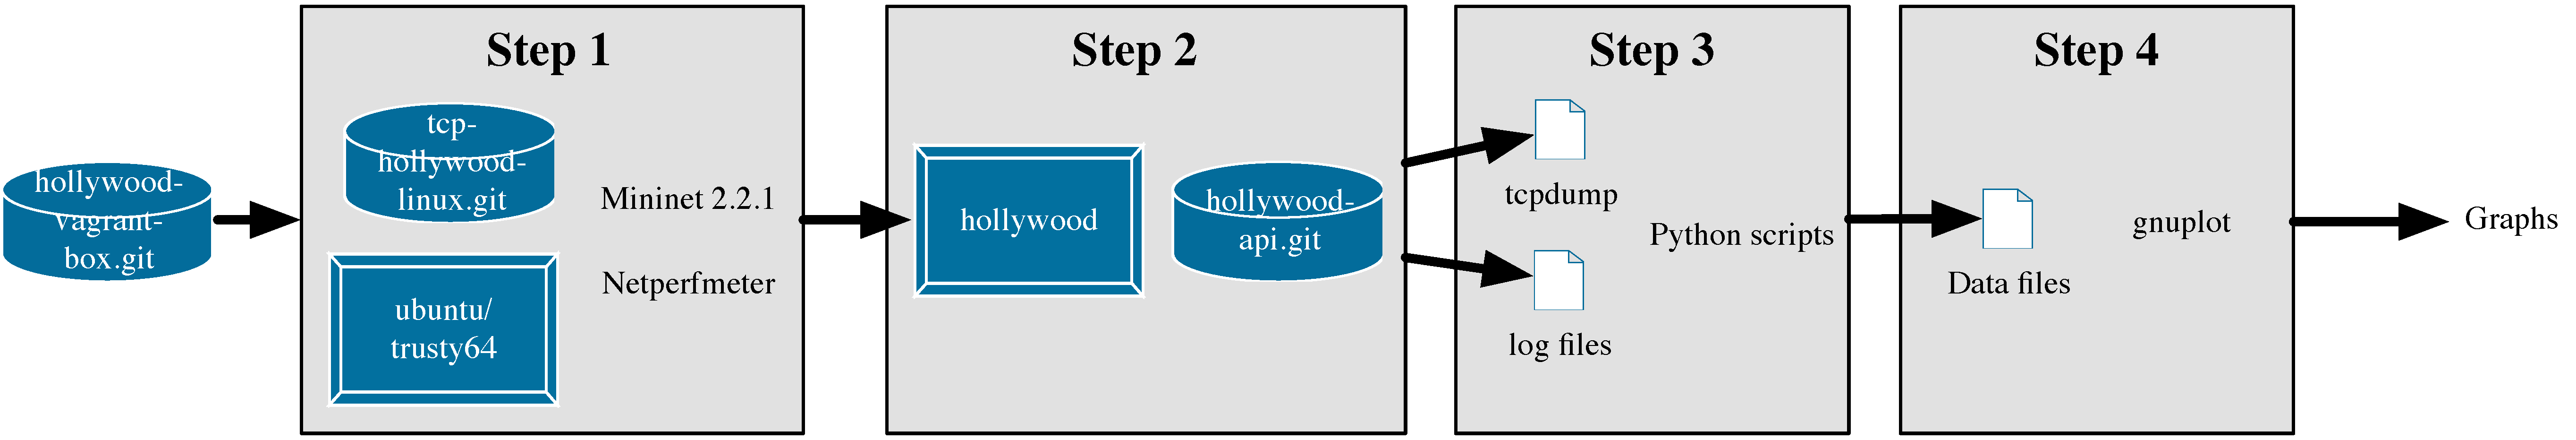
\includegraphics[width=\linewidth]{figures/reproducibility-flow.pdf}
    \caption{Flow diagram from package to post-processing and presentation.}
   	\label{fig:reproducibility-flow}
\end{figure}

\begin{figure}[t!]
\scriptsize
\begin{Verbatim}[commandchars=\\\{\}]
\textbf{perf-voip-adsl-uk-pd150ms-i-tcph.aclient-out:}
  [1484911921.078497] Received message 0 (elapsed 0.031388)
  [1484911921.078528] Playout thread started
                      - playout starting in 150ms
  ...
  [1484911921.228644] Playout started!
  [1484911921.228666] Expired 0 (0.181557 since sending)
\textbf{perf-voip-adsl-uk-pd150ms-i-tcph.aclient-tcpdump:}
  .. seq 13616429:13616593, ack 2937995557 .. length 164
  .. ack 13616593 .. length 0
\textbf{perf-voip-adsl-uk-pd150ms-i-tcph.aclient-kernlog:}
  Hollywood (PR): sending TCP segment (seq: 13617085)
  ...
  Hollywood (PR): .. sending message seq 9
  Hollywood (PR): .... time in queue: 0.000046677
  Hollywood (PR): .... one way delay: 0.011486000
  Hollywood (PR): .... play-out delay: 0.150000000
  Hollywood (PR): .... total time estimate: 0.161532677
  Hollywood (PR): .... message lifetime: 0.150000000
  Hollywood (PR): **** message expired!!
  Hollywood (PR): ++++++ no replacement found
\end{Verbatim}
\normalsize
\caption{Sample output of performance evaluation run}
\label{fig:perf-eval-output}
\end{figure}

The steps needed to reproduce our results, illustrated by
Figure~\ref{fig:reproducibility-flow}, are as follows. The code used to generate
this paper, including the performance evaluation results, is available
at~\url{https://github.com/lumisota/ifip-otcs-hollywood}.

\begin{enumerate}
  \item \emph{Build hollywood-0bb4a643.box:}
     Create Vagrant box, \emph{hollywood-0bb4a643.box}, that runs the TCP Hollywood
     kernel, with Mininet and other dependencies installed. Vagrant packages
     virtual machines into \emph{boxes}, alongside a \emph{Vagrantfile} that
     describes the box and sets a particular environment. The Makefile and other
     code required to build this box is located at
     \url{https://github.com/lumisota/hollywood-vagrant-box}.

    The Vagrant box used for the evaluations in this paper uses Ubuntu 14.04 (\texttt{ubuntu/trusty64}), and can be generated by running \texttt{make hollywood-0bb4a643.box}. Additional required software is installed via the \texttt{bin/box-setup.sh} script, and includes:
    % The base box (i.e., the bare initial box)
    % uses Ubuntu 14.04 (\texttt{ubuntu/trusty64}). The following is then
    % installed on this base box:
    \begin{itemize}
      \small{
      \item Mininet version 2.2.1, for network simulation;
      \item netperfmeter version 1.6.1, for cross-traffic generation;
      \item dependencies, such as gcc, for building the kernel;
      \item dependencies for the intermediary layer and cross-traffic
            generation tools.
            }
    \end{itemize}
    Once installed, \texttt{bin/tcph-install.sh} downloads, builds, and
    installs, TCP Hollywood kernel source code from~\cite{hollywood-src}; it
    also modifies the bootloader toward the newly installed kernel. After
    additional maintenance, the setup script terminates having packaged a
    complete box for use with Vagrant.

    % after reducing the size of the virtual machine (e.g., by clearing the package manager's caches),
    % and the box is packaged for use with Vagrant.

\balance
    \item \emph{Perform emulated experiments:}
          A clean copy of \texttt{hollywood-0bb4a643.box} is used for each
          performance evaluation to prevent any order effects that
          might result from earlier runs. The TCP Hollywood API
          (revision \texttt{e7536f0}, dated 16 January 2017, from \url{https://github.com/lumisota/hollywood-api/})
          is installed within the running
          virtual machine, along with the script
          \texttt{evaluations/perf-voip-adsl.py}. That script uses the Mininet
          Python API to setup the and run each evaluation, and is parameterized
          to specify the play-out delay, cross-traffic class, and TCP version
          (i.e., standard TCP or TCP Hollywood), as described in Section \ref{sec:perfeval}. Each run
          produces a set of output files, in the format shown in Figure
          \ref{fig:perf-eval-output}.

          File \texttt{aclient-out} logs application play-out events, and the
          % showing when play-out begins,
          and the state of messages (i.e., whether expired, or is playable) at
          each play-out interval. This data is used to derive the timely goodput
          in Figures \ref{fig:voip-150-tg}, \ref{fig:voip-110-tg}, and
          \ref{fig:voip-60-tg}; also message latency and playout data in Figures
          \ref{fig:voip-150-tcp}, \ref{fig:voip-150-tcph},
          \ref{fig:voip-110-tcp}, \ref{fig:voip-110-tcph},
          \ref{fig:voip-60-tcp}, and \ref{fig:voip-60-tcph}.

          File \texttt{aclient-tcpdump} is a \texttt{tcpdump} captured
          at the application client
          %, and contains the incoming TCP segments.
          % This provides the information needed to
          % determine which segments are retransmitted.
          to identify retransmitted segments. File \texttt{aclient-kernlog} is a
          copy of the client's \texttt{/var/log/kern.log}, to which TCP
          Hollywood outputs status messages when performing inconsistent
          retransmissions.  Collectively, these files contain the data use for
          segments plots in Figures \ref{fig:voip-150-tcp},
          \ref{fig:voip-150-tcph}, \ref{fig:voip-110-tcp},
          \ref{fig:voip-110-tcph}, \ref{fig:voip-60-tcp},
          \ref{fig:voip-60-tcph}, and \ref{fig:voip-comparison}.
          Remaining output files, such as output of the cross-traffic generation
          tools, are used for debugging. They play no role in the results
          presented in this paper.

    \item \emph{Process and output results:}
          Python scripts convert the output from the tests into data
          files formatted for visualisation tools. The time for each test
          consists of a two-minute simulation, as well as the time to setup and
          teardown virtual machines. The separation between visualisation and
          data generation eases analysis and visualisation by reducing wait
          times and increasing flexibility.
          % (rather than having the performance evaluations output plottable  data
          % directly) allows for the visualisation of the output to be changed,
          % without requiring the performance evaluations to be rerun.
\end{enumerate}

The combination of mininet and Vagrant provides for a clean environment for
reproducible network protocol evaluations, allowing scripting with standard Unix
tools. There is also a high complexity in composing all the pieces, and in
managing the scripts that automate analysis of the results. We strongly support
attempts to make results reproducible. To this end, we make TCP Hollywood source
code available as a template for further development and evaluation. However, we
%feel the need to
caution that the sheer number of components to the evaluation environment, and
the opaque nature of some of the tools, is such that there are doubts about the
\emph{long-term} reproducibility of results in this paper using the tools
described. The need for clear documentation of the algorithms is not diminished
by the availability of testing scripts, source code, and virtual machine images.
In the short term, however, those tools can be a highly effective way of
distributing runnable artefacts.
